\Chapter{Modèle basé sur les vitesses de dérive pour les plasmas froids}
\chaptermark{Vitesses de dérive pour les plasmas froid}

\label{AnnexeC}

\begin{refsection}
\section*{L'approche par vitesses de dérive pour les plasmas
froids}
\label{vitessesDerivePlasmaFroid}
Les équations de TOKAM2D ne décrivent
pas non plus l'interaction collisionnelle des particules chargées avec la
population neutre, essentielle dans la physique des plasmas froids. Dans les
régions non magnétisées, l'hypothèse de forte magnétisation sur laquelle se
base l'approximation des vitesses de dérive n'est plus valable. Pour étendre le
domaine de validité du modèle, on peut cependant dériver une nouvelle
expression des vitesses de dérive qui tient alors compte de l'interaction
avec les neutres. Les équations forment une sorte de combinaison entre les
équations du transport magnétisé et celles du modèle de Dérive-Diffusion.

Reprenons l'équation du moment pour une espèce d'indice $\alpha$ :

\begin{equation}
\label{2-MaplEqMoment}
\frac{\text{d}\mathbf{u}_\alpha}{\text{dt}}+
\nu_\alpha\mathbf{u}_\alpha+\omega_{c\alpha}\mathbf{b}\times\mathbf{u}_\alpha=
-\frac{q_\alpha}{m_\alpha}\left(\nabla \Phi +\frac{\nabla p_\alpha}{q_\alpha n_\alpha}\right)
\end{equation}

En prenant le produit vectoriel de \eqref{2-MaplEqMoment} et du champ
magnétique,  on peut éliminer le terme de
Lorentz $\omega_{c\alpha}\mathbf{b}\times\mathbf{u}_\alpha$ :

\begin{equation}
\label{2-MaplVitesse}
\mathbf{u}_\alpha=\frac{q_\alpha}{m_\alpha}(\nu_\alpha\puissance{2}+\omega_{c\alpha}\puissance{2})\puissance{-1}
\left[-\frac{q_\alpha}{m_\alpha}\left(\nabla \Phi +\frac{\nabla
p_\alpha}{q_\alpha
n_\alpha}\right)-\frac{\text{d}\mathbf{u}_\alpha}{\text{dt}}\right]
\end{equation}

 \begin{figure}[!htbp]
    \centering
    \subfigure[]{\label{2-CarteDensiteMapl}
    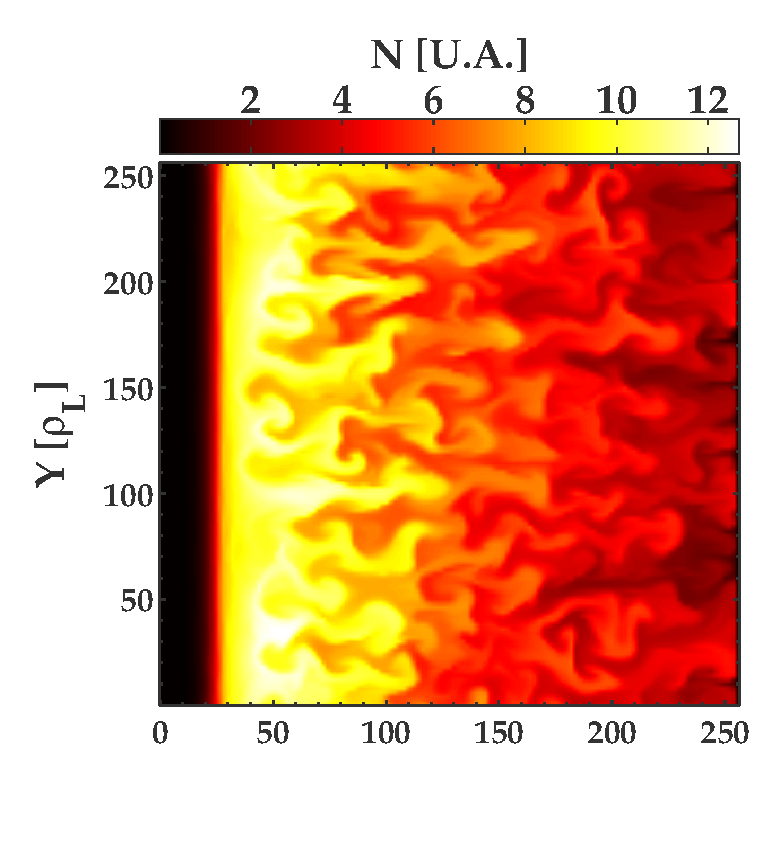
\includegraphics[height=8cm]{figures/2-CarteDensiteMapl.eps}}
    \subfigure[]{\label{2-CartePotentielMapl}
    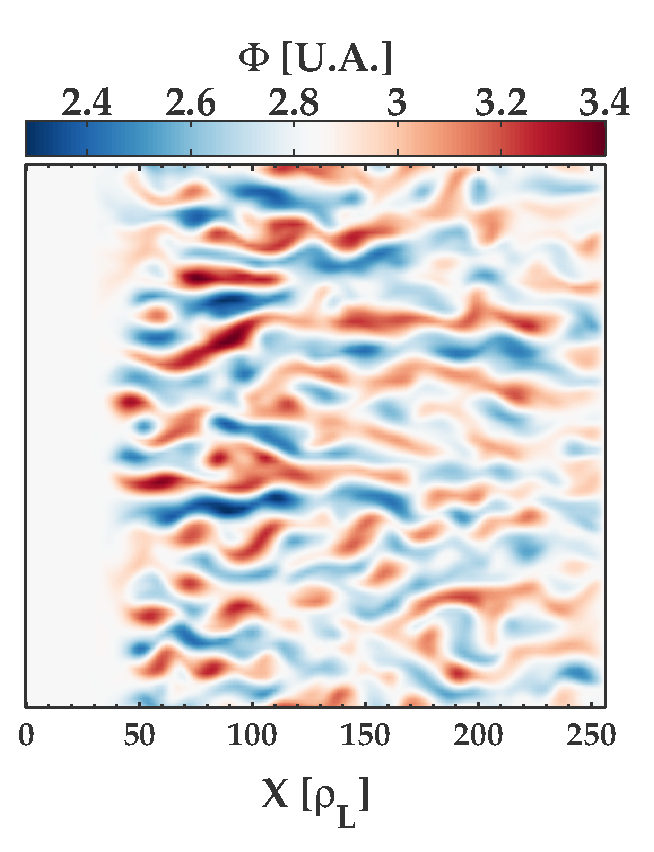
\includegraphics[height=8cm]{figures/2-CartePotentielMapl.eps}}
    \caption{Cartes de densité \subref{2-CarteDensiteMapl}~et de potentiel
    \subref{2-CartePotentielMapl}.}
	\end{figure}
	\end{refsection}
	\lipsum[40]{20}